
%General
Many developments in the past years increased the understanding of Relative Alchemical Free Energy (RAFE) calculations on an atomistic level significantly. Work on new RAFE applications exemplifies how more complex transformations such as scaffold hopping or the sampling of multiple end states from one simulation can be achieved. \cite{knight2011, Wang2017}
Recent developments on the methodological side improve the statistical robustness and the automatization of RAFE methods such that they can be applied for industrial purposes like virtual high-throughput screenings of drug compounds (vHTS). \cite{Cournia2017, Stroet2018, Jespers2019, Heinzelmann2021}

However, the choice of the different components for a free energy calculation is still non-trivial. Besides choosing an estimator such as  TI, the Zwanzig equation or BAR, or the sampling methodology, multiple options already exist for how to represent the different end states (i.e.: molecules) of interest during a simulation. \cite{Zwanzig1954, Kirkwood1935, Bennett1976}

%% Single, Hybrid and dual topology
%%% The Theoretic problem
In a RAFE calculation, one challenge to the structure of the model is to represent two (or multiple) end states in the subsequent simulation(s). This representation needs to provide accurate information of each end state at each sampling time step, which can be used in the final free energy estimation. 

%%% The solutions in application
Several possible methods were proposed in the past to build a coordinate and topology space in order to fulfill this requirement. 
However, the terminology is not very clear. Often, terms are used ambiguously, and different perspectives can be used to approach the topic. \cite{Boresch1999, Rocklin2013, Fleck2021} 
Historically, two approaches emerged, which were called single topology \cite{Pearlman1991, Pearlman1994, Hansen2013, Wang2017} and dual topology \cite{Pearlman1991, Gao1989, Sidler2016}.

To distinguish these two approaches, we would like to provide a perspective on the methodology based on the difference in the respective coordinate space, as this might lead to clearer categories. This perspective might differ from the initial historic naming, but it might prove more robust for clearly defining the differences between the different approaches. Here, the single topology approach in a strict definition contains a single set of coordinates for both end states. The dual topology approach contains a separate set of coordinates for each end state and, therefore, can be seen as the opposite extreme of the single topology approach. Three sub flavors for the dual topology approach could be identified in the literature: linked, separated and unconstrained.
A  hybrid single-dual topology approach was recently described \cite{Jiang2019} and used before in many other schemes. This approach combines the two extreme approaches(i.e.: single and dual topology) and forms an intermediate to these approaches (Figure \ref{fig:Topology Types}). The different approaches vary in their sampling efficiency and the capability of representing different complex transformations.


\begin{figure}[h!]
    \centering
    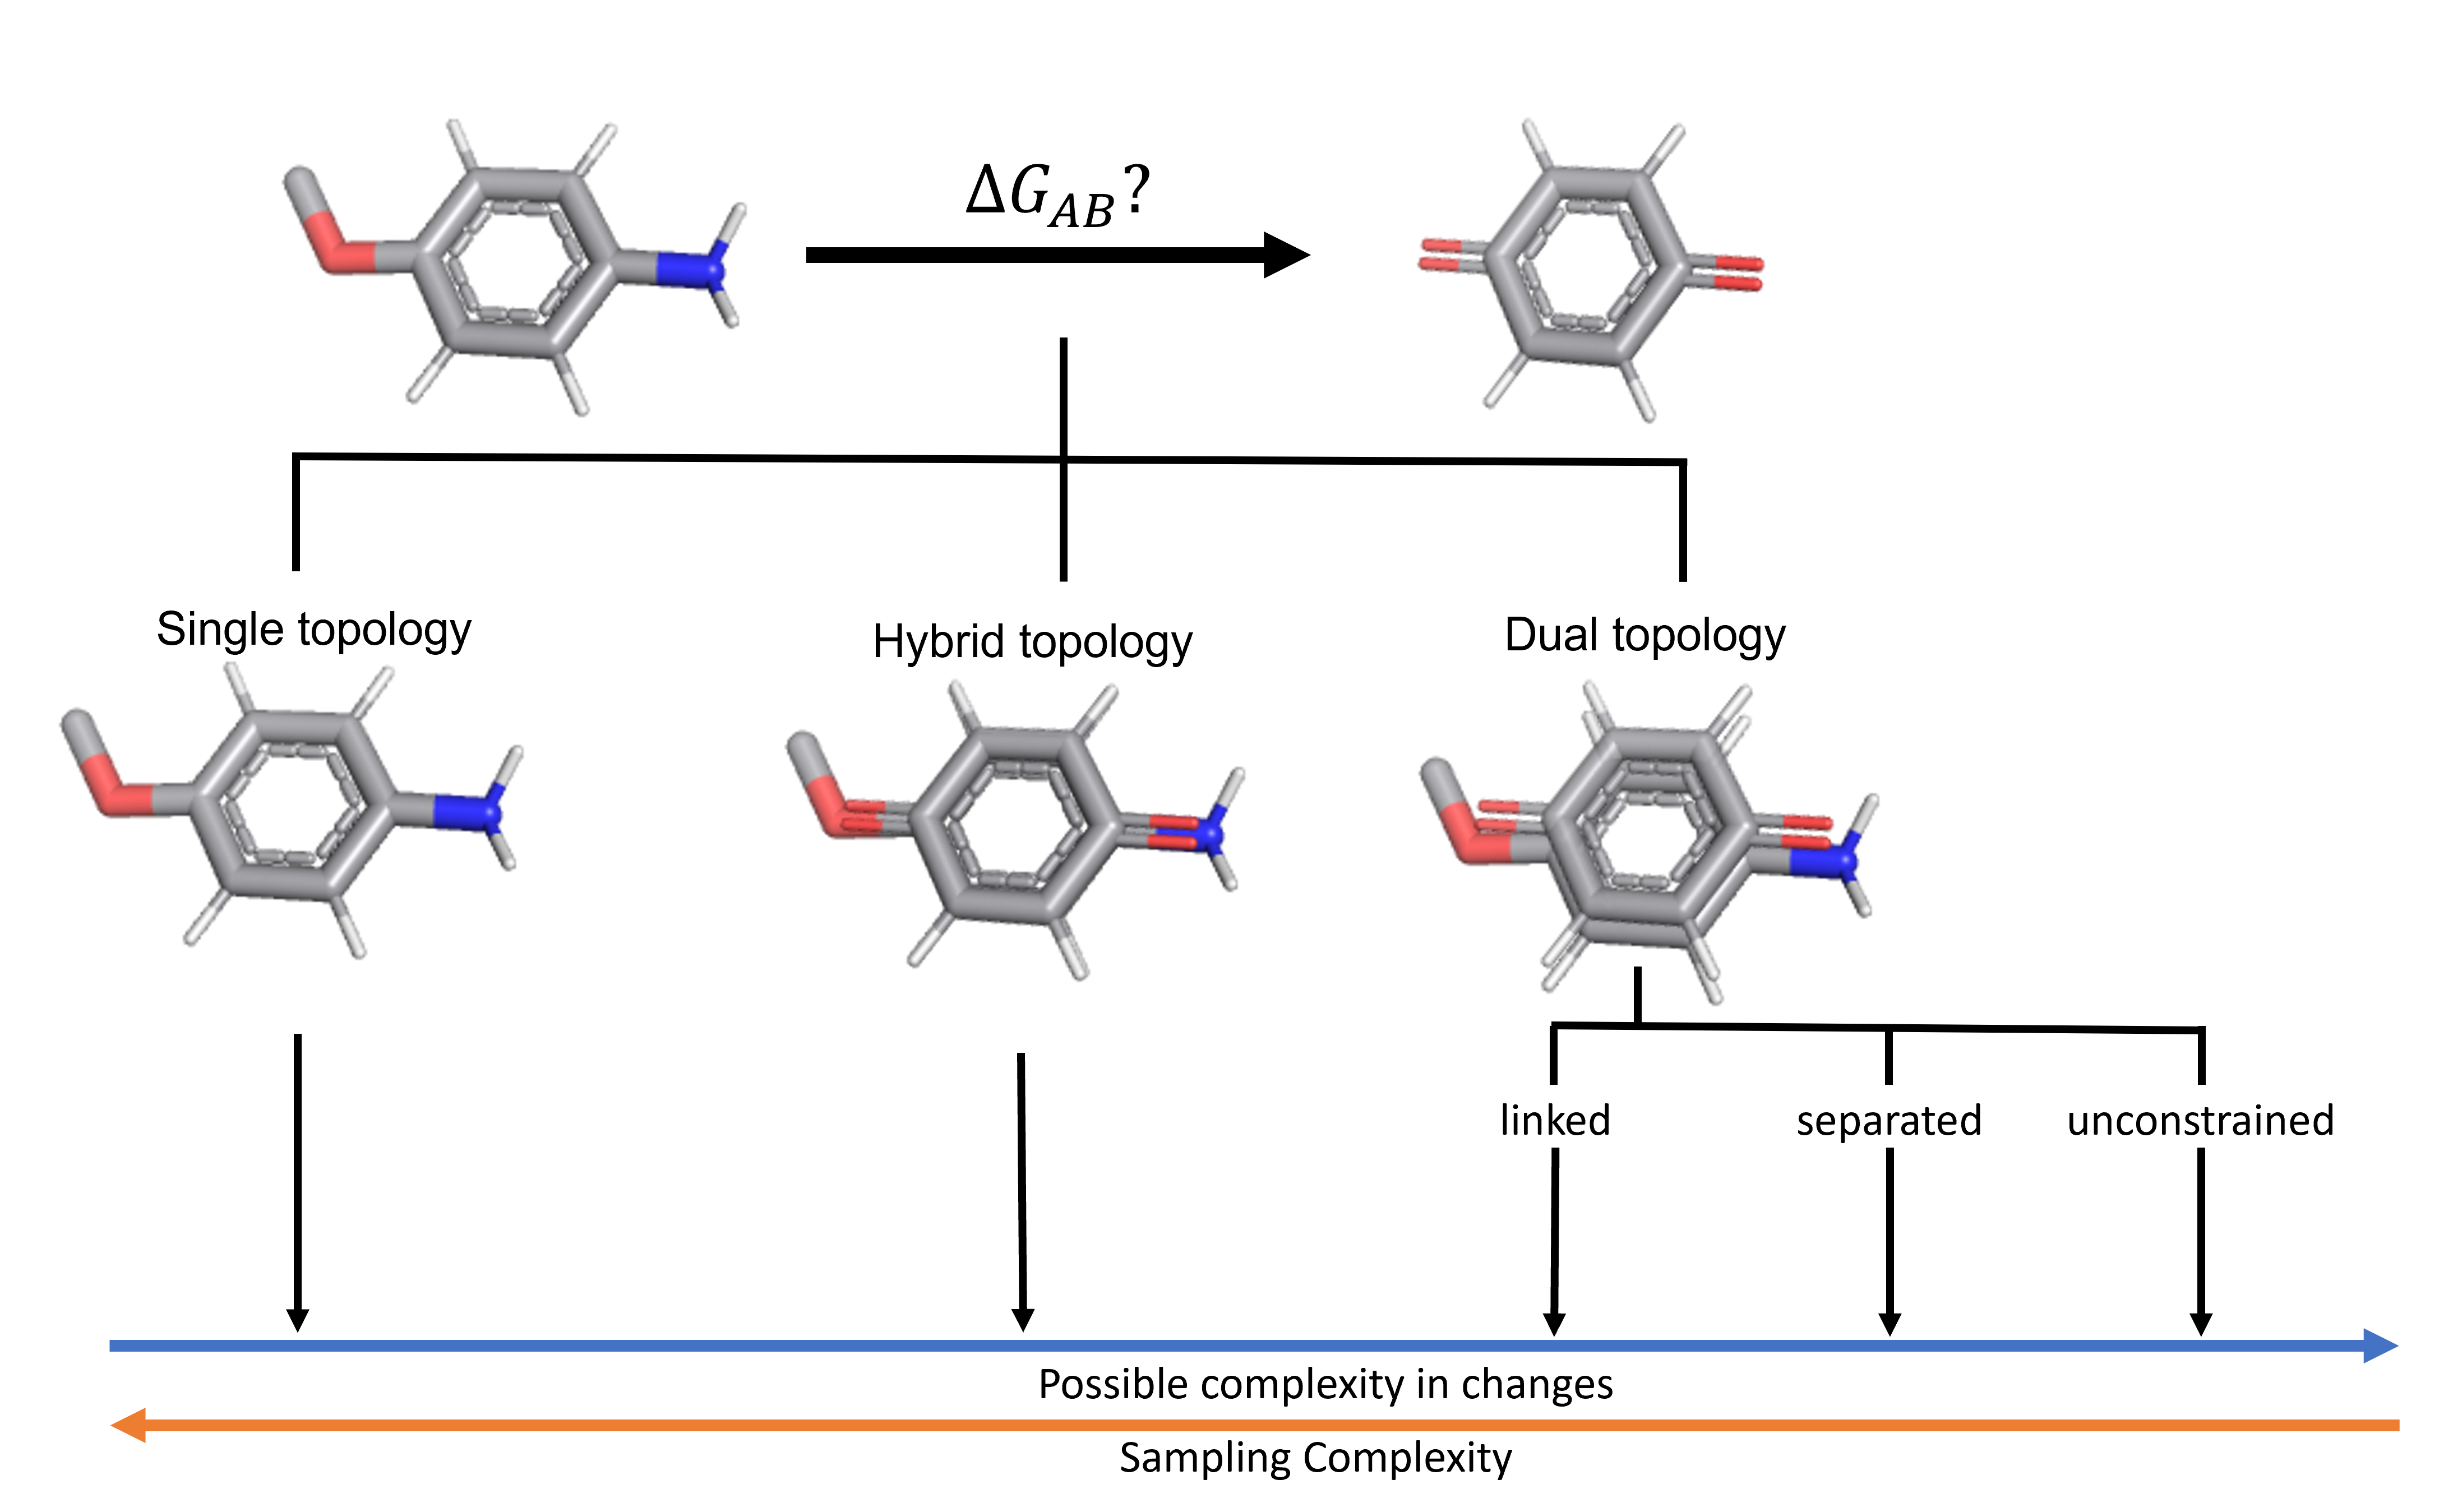
\includegraphics[width=\linewidth]{fig/theory/landscape_of_simulationApproaches.png}
    \caption{Three approaches for end-state representations can be distinguished from a coordinate space perspective for relative free energy calculations. The single topology approach contains a single set of coordinates for all end states. The dual topology approach contains separate sets of coordinates for each end state respectively. Finally, the hybrid topology approach combines atoms of identical substructures into one coordinate and separates atoms that differ in the end states. Therefore, it is an intermediate of the other two approaches. The dual topology approach can be subdivided into free flavors based on literature: linked, separated, and unconstrained. The linked dual topology approach is closest to the single topology approach, as the end state coordinate overlap is enforced via direct spatial restraints. The separated approach is mainly connecting the molecules indirectly by restraining them spatially to the same area. Finally, the unconstrained approach does not restrain the molecules at all and is therefore also the most sampling complex approach.}
    \label{fig:Topology Types}
\end{figure}

%%% single topology
\subsection{Single Topology}
%%%%Coordinate space
The single topology approach was first used by \textit{Joergensen et al.} to calculate the relative free energy of hydration for Methanol and Ethane. The approach was termed as such by \textit{Pearlman et al.} and refers to only swapping atom types of a system between the two end-states. \cite{Jorgensen1985, Pearlman1991, Pohorille2010, Jespers2019}
Therefore, both end-states are represented by a single set of coordinates, limiting the possible structural differences used with this method.

A single topology approach in this definition is constructed as follows:
\begin{align*}
    \text{given a state A and B:}\\
    n_{single}^{AB} &= n_A = n_B\\
    \vec{r}_{single} &= \{\vec{r}_{AB_1}, \vec{r}_{AB_2}, ..., \vec{r}_{AB_{n_{AB}}}, \vec{r}_{env_1}, \vec{r}_{env_2}, ..., \vec{r}_{env_{n_{env}}}\}\\
    \vec{f}_{single} &= \{\vec{f}_{A_1}, \vec{f}_{A_2}, ..., \vec{f}_{A_{n_A}},\vec{f}_{B_1}, \vec{f}_{B_2}, ..., \vec{f}_{B_{n_B}}, \vec{f}_{env_1}, \vec{f}_{env_2}, ..., \vec{f}_{env_{n_{env}}}\}
\end{align*}
with n being the number of atoms, $\vec{r}$ the coordinate space vector and $\vec{f}$ the force vector. The end states A and B represent  the different end-states and the index env stands for the environment surrounding the end-states, which is not changing (i.e.: water solvatisation, protein, etc.).

%%%%Problems and solutions]
%%%%%%Sampling
In the past, the single topology approach showed the best sampling efficiency compared to other approaches, which can be explained by the reduced degrees of freedom in the coordinate space compared to the dual topology approach. \cite{Pearlman1994, Donnini2011, Yu2017, Fleck2021}

%%%%%Different Atoms
Challenging transformations for this approach are, for example, if an atom is not present in both states. Therefore, it is common to define the coordinate space as the union of all atoms and assign a non-interacting `dummy' state to the vanishing atom/s. \cite{Pearlman1994, Donnini2011, Yu2017, Fleck2021}
Different variants of `dummy' states are possible. Often, only the non-bonded interactions are removed from such atoms. However, it was studied by \textit{Fleck et al.}, how the bonded terms of `dummy' states influence the free energy calculations. \cite{Fleck2021}
Though the dummy atom approach allows changes in the number of atoms of the end states, it is challenging to build a system for complex structural changes such as scaffold hopping transformations.
However, recent developments showed that the single topology approach could realize complex transformations such as ring size changes or a ring-opening by employing special soft bond terms. The limitation of this approach is the necessary rearrangement of atoms or difficult dummy atom construction for very complex transformations that change whole molecule core structures or a large number of atoms.\cite{Wang2017} 


%%% hybrid topology
\subsection{Hybrid Topology}
In the past, some approaches termed single or dual topology could instead fit into a hybrid topology category, to separate the methodologies more clearly.
The hybrid category is an intermediate between single- and dual-topology approaches. Early studies with these approaches were published by \textit{Shobana et al.} for amino acid mutations in a more dual topology-like flavor and a more single topology-like approach by \textit{Eriksson et al.} for a base pair exchange in DNA simulations.\cite{Shobana2000, Eriksson1995}
The Hybrid Single-Dual-Topology approach was formally introduced by \textit{Jiang et al.} and focuses on building up a single topology core region. \cite{Jiang2019} It sets up the topology approach such that a single set of coordinates represents the common  core substructure, and the diverging parts of the structures are represented with individual coordinates like in a dual topology approach. \cite{Jiang2019}  

A hybrid topology approach in our definition can be constructed with the following rules:
\begin{align*}
    \text{given a state A and B:}\\
    n_{hybrid}^{AB} &= n_{AB}(A \cap B) + n_A(A \setminus B) + n_B (B \setminus A)\\
    %V(\vec{r}) &= V_A(\vec{r_{AB},\vec{r_{A}}})+V_B(\vec{r_{AB}, \vec{r_{B}}})+V_{env}(\vec{r_{env}})\\
    \vec{r}_{hybrid} &= \{\vec{r}_{AB_1}, \vec{r}_{AB_2}, ..., \vec{r}_{AB_{n_{AB}}}, \vec{r}_{A_1}, \vec{r}_{A_2}, ..., \vec{r}_{A_{n_{A}}}, \vec{r}_{B_1}, \vec{r}_{B_2}, ..., \vec{r}_{B_{n_{B}}},    \\ 
     &~~~\vec{r}_{env_1}, \vec{r}_{env_2}, ..., \vec{r}_{env_{n_{env}}}\}\\
    \vec{f}_{hybrid} &= \{\vec{f}_{A_1}, \vec{f}_{A_2}, ..., \vec{f}_{A_{n_{A}}},\vec{f}_{B_1}, \vec{f}_{B_2}, ..., \vec{f}_{B_{n_{B}}}, \vec{f}_{env_1}, \vec{f}_{env_2}, ..., \vec{f}_{env_{n_{env}}}\}
\end{align*}
with $n$ as the number of atoms, $\vec{r}$ the coordinate space vector and $\vec{f}$ the force vector. The end states A and B are the representatives for the different end-states and the index $env$ stands for the environment surrounding the end-states, which is not changing (i.e.: water solvatisation, protein, etc.).

%%%%%%
Hybrid approaches try to combine the benefits of single and dual topology to have a beneficial effect on the sampling efficiency from the single-topology region and allow complex transformations like in dual topology approaches. In an extreme case, these approaches end up in one of the two extreme approaches. \cite{Jiang2019}

%%%Dual Topology
\subsection{Dual Topology}
The dual topology approach keeps the transforming atom coordinates entirely separate and therefore contains two sets of coordinates for groups that are transformed in the end-states. This approach stands as contrary  to the single topology approach and was first introduced by \textit{Gao et al.} and termed as such by \textit{Pearlman et al.}. \cite{Gao1989, Pearlman1991}
The two sets of coordinates can not interact with each other and usually only share the same environment. \cite{Riniker2011, Rocklin2013}

A dual topology approach in our definition follows the following rules:
\begin{align*}
    \text{given a state A and B:}\\
    n_{dual}^{AB} &= n_A + n_B\\
    %V(\vec{r}) &= V_A(\vec{r_{A}})+V_B(\vec{r_{B}})+V_{env}(\vec{r_{env}})\\
    \vec{r}_{dual} &= \{\vec{r}_{A_1}, \vec{r}_{A_2}, ..., \vec{r}_{A_{n_{A}}}, \vec{r}_{B_1}, \vec{r}_{B_2}, ..., \vec{r}_{B_{n_{B}}},\vec{r}_{env_1}, \vec{r}_{env_2}, ..., \vec{r}_{env_{n_{env}}}\}\\
    \vec{f}_{dual} &= \{\vec{f}_{A_1}, \vec{f}_{A_2}, ..., \vec{f}_{A_{n_{A}}},\vec{f}_{B_1}, \vec{f}_{B_2}, ..., \vec{f}_{B_{n_{B}}}, \vec{f}_{env_1}, \vec{f}_{env_2}, ..., \vec{f}_{env_{n_{env}}}\}
\end{align*}
with $n$ as the number of atoms, $\vec{r}$ the coordinate space vector and $\vec{f}$ the force vector. The end states A and B are the representatives for the different end-states and the index $env$ stands for the environment surrounding the end-states, which is not changing (i.e.: water solvatisation, protein, etc.).

%%%% Sampling
The separated coordinates lead to more degrees of freedom, lowering the sampling efficiency compared to single topology approaches for simple transformations. In order to improve the sampling efficiency, it is common to apply spatial restraints to the end-state coordinate sets to prevent them from drifting apart from each other. \cite{Riniker2011, Mobley2006}

%%%% Transformation
A significant advantage of this approach is the straightforward setup of a system, even for more complex transformations, compared to the single and hybrid topology approaches. 

%%%% Problems and solutions
%%%% Restraint problem
\subsection{Restraint Problem}
Regarding the spatial restraints improving the sampling efficiency for dual topology approaches, multiple sub approaches can be distinguished:
an unconstrained approach \cite{Henin2004, Carvalho2021}, an approach with constraints from one end-state to another end-state in order to maximize the end-state shape overlap, which will be referred to as a linked dual topology approach \cite{Riniker2011, Sidler2016}, and an approach with constraints to the environment which will be referred to as separated dual topology. \cite{Mobley2006, Rocklin2013}
The linked dual topology can be the most sampling efficient one from these three approaches if the transformation is comparably simple (i.e., no largely different binding modes of the two end states induced by reorientation or large conformational differences). The separated dual topology approach is the second most efficient approach but has the advantage of allowing more complex transformations, such as the reorientation of one end state in a binding pocket. The unconstrained case finally follows these approaches. \cite{Mobley2006}

%%%% Automatization
With the growing need of automatization for free energy calculations, questions arise on how to realize this endeavour. Although there are tools to automatically set up single topology RAFEs, such as FESetup\cite{Loeffler2015}, the dual topology approaches are the easiest ones to be automatized, as any change can be easily realized without the requirement of any atom mapping. \cite{Rocklin2013}
For the unconstrained dual topology case, an automatic procedure setting up RAFE simulations exists in the package pyFEP. \cite{Carvalho2021}. The linked dual topology approach of the QligFEP pipeline provides an automatic system generation part for their methodology. This pipeline sets distance restraints onto identical substructure regions of the end states. \cite{Jespers2019}

Nevertheless, with the increase of the complexity of the transformation for RAFE in the field (i.e., especially in the form of scaffold hopping), approaches need to come up with more flexible ways for restraining the end-states with spacial restraints.

%outlook
This work will focus on the linked dual topology approach and the challenge of finding reasonable restraints that do not remove essential parts of the phase space for small molecules, representing molecules from drug discovery that contain a rigid core. 
We will construct an algorithm that provides reasonable restraints for the linked dual topology approach for pairwise RAFE methods. Further, this algorithm will be expanded to solve the same problem for multistate RAFE methods (resulting in a linked multi-topology approach). Finally, we will analyze the sampling behavior and performance of the approach with hydration-free energy calculations. The algorithm is implemented in a  python package (github: https://github.com/rinikerlab/restraintmaker) which can be used as a scripting library or with a GUI via PyMOL. \cite{DeLano2020}